% !TeX root = ../main.tex

\section{CI/CD}
    \begin{frame}{Mobile Application Development Lifecycle}
        \begin{columns}[onlytextwidth]
            \begin{column}{0.4\textwidth}
                \begin{itemize}
                    \item Pianificazione
                    \item Progettazione
                    \item Sviluppo
                    \item Stabilizzazione
                    \item Release
                    \item Monitoring
                \end{itemize}
            \end{column}
            \begin{column}{0.6\textwidth}
                \begin{figure}[H]
                    \centering
                    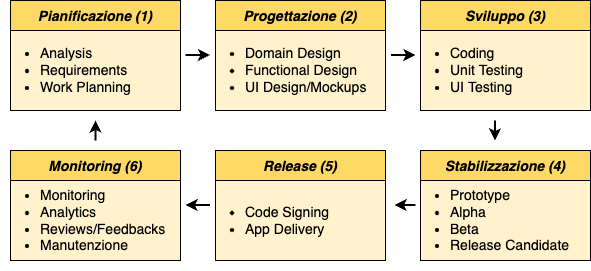
\includegraphics[width=1\textwidth]{img/tesi-2-Page-9.drawio.png}
                \end{figure}    
            \end{column}
       \end{columns}
    \end{frame}


%    \begin{frame}{Pipeline Obiettivo}
%        \begin{itemize}
%            \item I task del processo a cui sono applicate le tecniche di Continuous Integration e Continuous Delivery sono \textit{Sviluppo}, \textit{Stabilizzazione} e \textit{Release}.
%            \item Non esiste il concetto di deployment automatizzato nel mondo delle applicazioni mobile: l'applicazione viene rilasciata tramite pubblicazione sull'apposito store e l'utente effettua in un secondo momento l'installazione sul proprio dispositivo.
%            \item Dato il vincolo tecnologico del framework KMM per lo sviluppo della applicazione, la pipeline è stata progettata utilizzando come caso d'uso l'applicazione base generata con il plugin Gradle KMM.
%        \end{itemize}
%    \end{frame}

    \begin{frame}{Branching Model}
        \begin{columns}[onlytextwidth]
            \begin{column}{0.5\textwidth}
                \begin{itemize}
                    \item Fondamentale per l'efficacia del processo progettato
                    \item Basato su GitFlow
                    \item Branch principali:
                    \begin{itemize}
                        \item \textit{dev} (alpha)
                        \item \textit{test} (beta)
                        \item \textit{main} (prod)
                    \end{itemize}
                \end{itemize}
            \end{column}
            \begin{column}{0.5\textwidth}
                \begin{figure}[H]
                    \centering
                    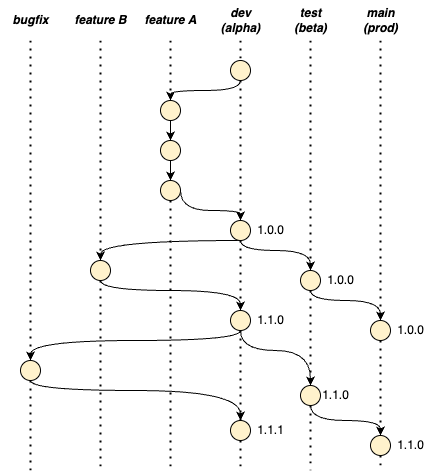
\includegraphics[width=0.9\textwidth]{img/tesi-13-branching.drawio.png}
                \end{figure}
            \end{column}
        \end{columns}
    \end{frame}
    
    \begin{frame}{Pipeline Obiettivo}
        \begin{figure}[H]
            \centering
            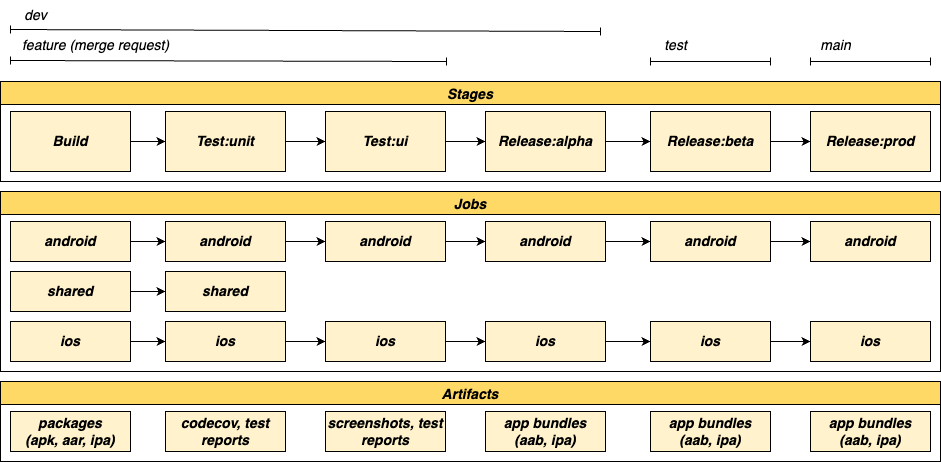
\includegraphics[width=1\textwidth]{img/tesi-2-Page-12.drawio.png}
        \end{figure}  
    \end{frame}

    \begin{frame}{Continuous Integration}
    \begin{itemize}
        \item Integrazione molto frequente di piccole modifiche al flusso di sviluppo principale.
        \item Ad ogni modifica il codice attraversa la pipeline progettata per validare compilazione, packaging, business logic e interfaccia grafica.
        \item Coinvolge i branch \textit{dev}, \textit{feature} e \textit{bugfix} (tramite merge request).
        \item Stages:
            \begin{itemize}
                \item \textbf{Build} - Fase di compilazione e packaging.
                \item \textbf{Test}
                \begin{itemize}
                    \item \textit{Unit Testing} - Fase di testing della business logic.
                    \item \textit{UI Testing} - Fase di testing della interfaccia grafica.
                \end{itemize}
            \end{itemize}
        \end{itemize}
    \end{frame}

    \begin{frame}{Continuous Delivery}
        \begin{itemize}
            \item Rilascio molto frequente di piccole modifiche al flusso di sviluppo principale.
            \item Ogni piccola modifica apportata al codice se passa con successo la fase di integrazione deve essere rilasciata come nuova versione della applicazione.
            \item Coinvolge i branch \textit{dev}, \textit{test} e \textit{main}.
            \item Stages:
            \begin{itemize}
                \item \textbf{Release}
                \begin{itemize}
                    \item \textit{Alpha} - Fase di rilascio a scopo di test interno.
                    \item \textit{Beta} - Fase di rilascio a scopo di test esterno.
                    \item \textit{Prod} - Fase di rilascio a scopo di pubblicazione sugli store.
                \end{itemize}
            \end{itemize}
        \end{itemize}
    \end{frame}

    \begin{frame}{Continuous Inspection}
        \begin{columns}[onlytextwidth]
            \begin{column}{0.4\textwidth}
                \begin{itemize}
                    \item \textbf{Test}
                        \begin{itemize}
                            \item \textit{Unit Testing} - Fase di testing della business logic.
                            \item \textit{UI Testing} - Fase di testing della interfaccia grafica.
                        \end{itemize}
                    \item \textbf{Analysis}
                        \begin{itemize}
                            \item \textit{SAST} - Fase di analisi statica del codice.
                            \item \textit{SCA} - Fase di analisi delle dipendenze.
                            \item \textit{Sonar} - Fase di upload dei report su SonarQube.
                        \end{itemize}
                \end{itemize}
            \end{column}
            \begin{column}{0.6\textwidth}
                \begin{figure}[H]
                    \centering
                    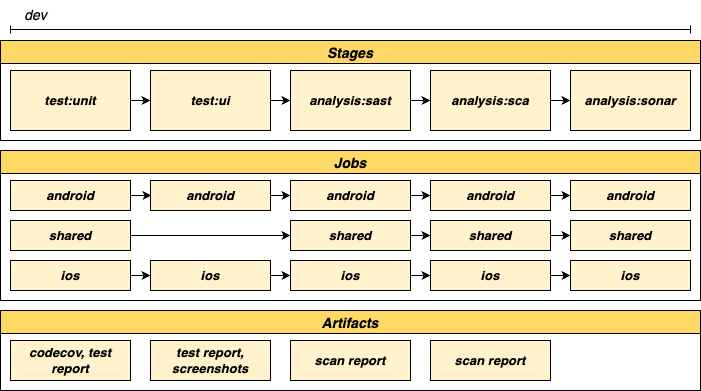
\includegraphics[width=1\textwidth]{img/tesi-2-Page-19.drawio.png}
                \end{figure}
            \end{column}
            
        \end{columns}
    \end{frame}